\section{PCA}



\begin{figure}[h!]
  \begin{center}
    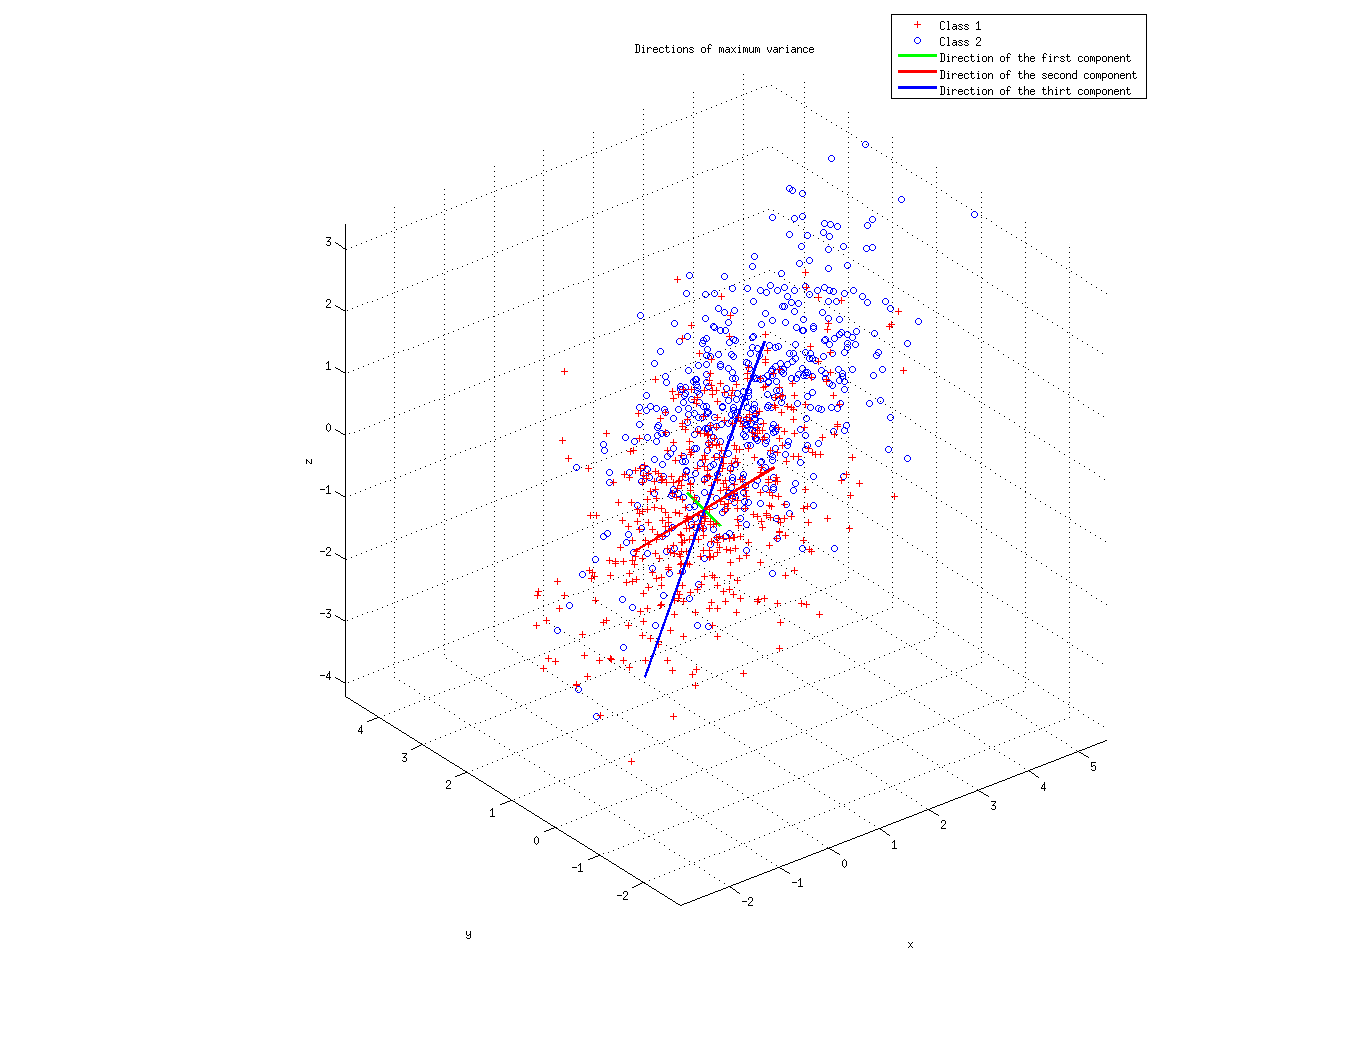
\includegraphics[width=0.75\textwidth]{./figures/4_Components}
    \caption{Die Richtungen der maximalen Varianz für die Daten, Richtungen mit den Eigenwerten Skaliert.}
    \label{fig:4_components}
  \end{center}
\end{figure}

\begin{figure}[h!]
  \begin{center}
    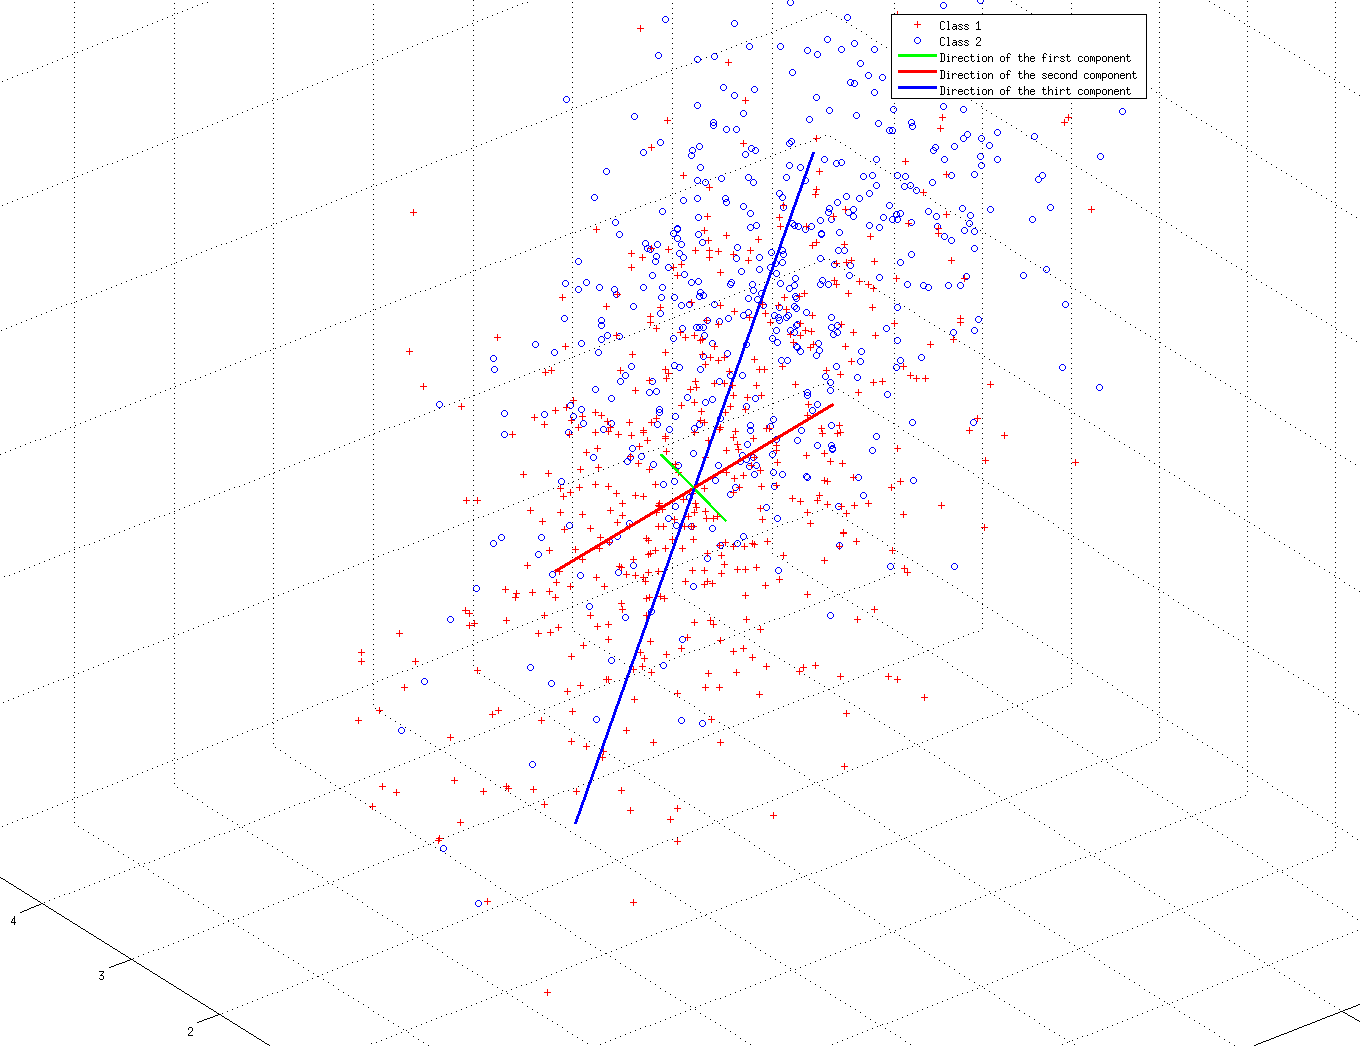
\includegraphics[width=0.75\textwidth]{./figures/4_Components_zoom}
    \caption{Die Richtungen der maximalen Varianz für die Daten, Richtungen mit den Eigenwerten Skaliert und vergrößert.}
    \label{fig:4_components_zoom}
  \end{center}
\end{figure}
Abbildung~\ref{fig:4_components} zeigt die Wolke aus den Punkten, wobei die Punkte der beiden Klassen getrennt dargestellt werden, und die zu den Daten gehörenden Hauptkomponenten.
Abbildung~\ref{fig:4_components_zoom} zeigt das selbe Bild nur etwas Vergrößert.\newline
 
\begin{figure}[h!]
  \begin{center}
    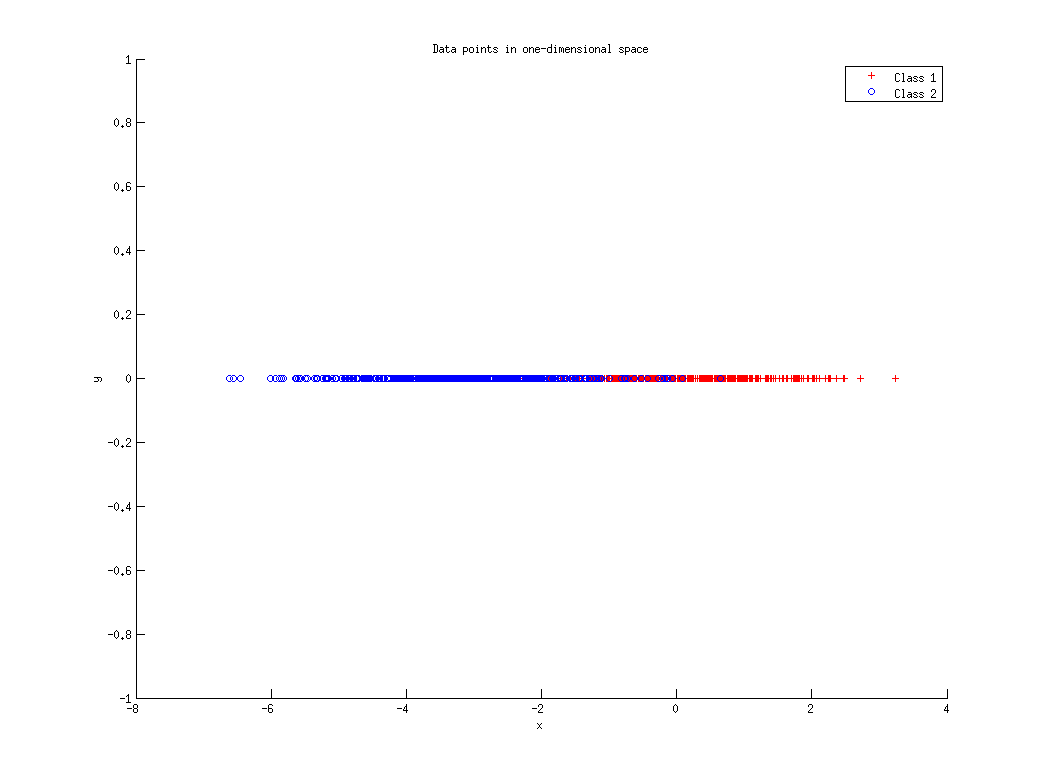
\includegraphics[width=0.75\textwidth]{./figures/4_one_dim}
    \caption{Projektion der Daten in eine einzige Dimension.}
    \label{fig:4_one_dim}
  \end{center}
\end{figure}

\begin{figure}[h!]
  \begin{center}
    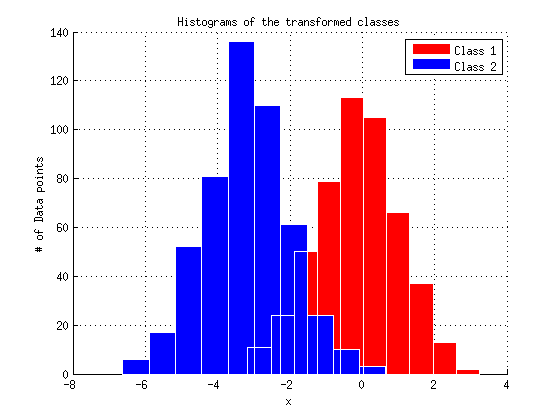
\includegraphics[width=0.75\textwidth]{./figures/4_Histogram}
    \caption{Histogram der Projezierten Daten.}
    \label{fig:4_Histogram}
  \end{center}
\end{figure}


Durch die PCA können die Daten nicht ihn ihr Wahrscheinlichkeitsverteilung beeinflusst werden.

Unser Thrashold berechnet sich in unserem Beispiel zu -1.1983 die Performance liegt bei 88.5\% 


%Man erkennt, dass die Gewichte die Bereiche in den Patterns hervorheben, die zum Unterscheiden der Patterns wichtig sind (\emph{Features}). Diese Bereiche haben in den Gewichtsmatrizen den gleichen Wert. Vergleicht man Abbildungen \ref{fig:4_patterns} und \ref{fig:4_weight}, fällt sofort auf, dass die Bereiche, die in den Patterns unterschiedlich sind (und damit die wichtigsten Merkmale) in den Gewichtsmatrizen besonders herausstechen. Dabei haben die Elemente, bei denen sich die Patterns \texttt{8} und \texttt{3} unterscheiden einen anderen Wert als z.B. die Elemente, bei denen sich die Patterns \texttt{8} und \texttt{0} unterscheiden. Dadurch kann das neuronale Netzwerk durch richtiges gewichtetes Addieren (Hidden Layer $\rarrow$ Output Layer) Ausgänge erzeugen, von denen bei richtig erkannten Zeichen jeweils nur einer aktiv wird, sprich Output-Neuron \texttt{0} reagiert z.B. auf einen hohen Wert von Hidden-Neuron 1 \emph{und} einen hohen Wert von Hidden-Neuron 2. Das passiert, wenn die Elemente, bei denen die Gewichte hoch sind (in Abb.~\ref{fig:4_weights} weiß) ebenfalls hoch sind (in Abb.~\ref{fig:4_patterns}), was für Daten, die das Zeichen \texttt{0} repräsentieren zutrifft.

